\section{Kiến trúc của trình thông dịch}
\begin{figure}[h]
    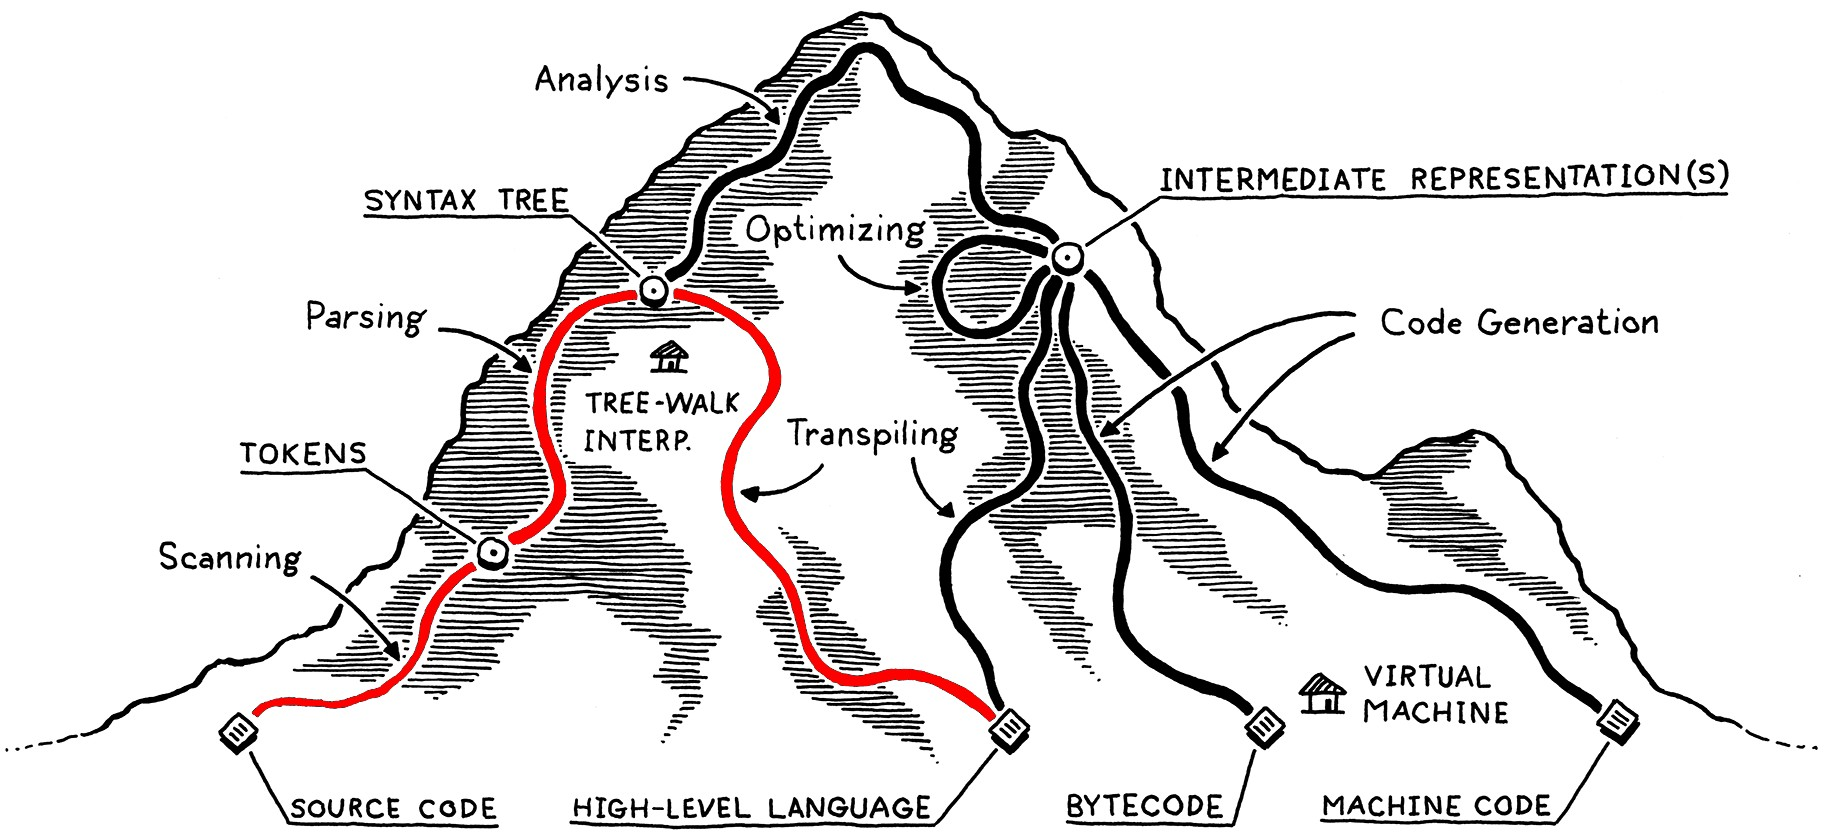
\includegraphics[scale=0.24]{interpreter.jpg}   
    \centering
    \caption{Các giai đoạn khi phân tích chương trình} 
    \label{fig:stages}
\end{figure}

Quá trình phân tích một ngôn ngữ được hình dung giống như leo núi. Bắt đầu từ dưới cùng với chương trình nguồn (chỉ là văn bản với chuỗi các ký tự thô), qua mỗi giai đoạn phân tích chương trình và chuyển đổi nó thành dạng biểu diễn cao cấp hơn, nơi mà ngữ nghĩa (những gì người lập trình muốn máy tính) trở nên rõ ràng hơn. Sau đó trình dịch nói chung chuyển đổi nó thành dạng biểu diễn mà máy tính có thể thực hiện (xuống núi) bằng nhiều cách khác nhau. Trình thông dịch lựa chọn đường "xuống núi" (thực thi chương trình) ngay sau khi có cây phân tích cú pháp (syntax tree) như đường màu đỏ trong hình \ref{fig:stages} \cite{craftinginterpreters}. Chi tiết từng giai đoạn sẽ được chúng em trình bày bên dưới.

\subsection{Từ tố (\textit{token})}
    Những từ tố đơn giản được định nghĩa bằng cách đưa trực tiếp mẫu của
nó (như các định nghĩa về từ khoá, dấu toán học, ...). Những từ tố phức tạp
hơn sẽ được định nghĩa bằng biểu thức chính quy như tên, xâu, số và chú thích.
Phần phân tích từ vựng (lexical analyzer) phải có khả năng phân tích chương trình nguồn
và đưa ra được các từ tố như sau:

\chapter*{BẢNG KÝ HIỆU}
\addcontentsline{toc}{chapter}{BẢNG KÝ HIỆU}
\begin{longtable}{| c | c |}
\hline
\textbf{\textit{Từ viết tắt}} & \textbf{\textit{Từ gốc}} \\
\hline
\end{longtable}


    Từ vựng của Pandora được xác định không chỉ từ chữ cái (alphabet) và chữ số (digit), mà là hầu hết các ký tự trong bảng mã Unicode \cite{allen2012unicode}, cụ thể như sau:

    \regexdigit

    \regexalphabet

\noindent và các ký tự khác trong bảng mã Unicode.

    Khoảng trắng (\textbf{whitespace}) là bất kỳ chuỗi không trống nào chỉ chứa các ký tự có thuộc tính Unicode Pattern\_White\_Space \cite{web:unicode:report}, cụ thể là:
    \begin{itemize}
        \item{U+0009 (horizontal tab, '\textbackslash t')}
        \item{U+000A (line feed, '\textbackslash n')}
        \item{U+000B (vertical tab)}
        \item{U+000C (form feed)}
        \item{U+000D (carriage return, '\textbackslash r')}
        \item{U+0020 (space, ' ')}
        \item{U+0085 (next line)}
        \item{U+200E (left-to-right mark)}
        \item{U+200F (right-to-left mark)}
        \item{U+2028 (line separator)}
        \item{U+2029 (paragraph separator)}
    \end{itemize}
\noindent Pandora là một ngôn ngữ "dạng tự do", có nghĩa là tất cả các dạng khoảng trắng chỉ dùng để phân tách các từ tố trong ngữ pháp và không có ý nghĩa ngữ nghĩa.

    Tên \textbf{\textit{identifier}} trong Pandora được phân làm 2 loại: \textbf{non keyword identifier} hoặc \textbf{raw identifier}. \textbf{non keyword identifier} được tạo thành từ tập các kí tự nêu trên và không được là từ khóa (keyword). Trong khi đó, \textbf{raw identifier} có thể là tên hoặc từ khóa (có \textbf{r\#} ở phía trước để phân biệt với tên thường hay từ khóa), cụ thể như sau:

    \regexidentifier

\noindent Trong đó \textbf{XID\_Start} và \textbf{XID\_Continue} là các thuộc tính của ký tự trong Unicode liên quan đến tên (định danh). Chúng thường được sử dụng để xác định liệu một ký tự có thể là phần đầu hoặc phần thân của 1 định danh trong các ngôn ngữ lập trình hay không. Ngoài ra, 1 tên còn có thể chứa các biểu tượng cảm xúc (\textbf{EMOJI\_SYMBOL}).

    1 ký tự chữ (\textbf{character}) là 1 ký tự Unicode đơn được đặt trong 2 ký tự ' (dấu nháy đơn - U+0027), ngoại trừ chính U+0027, ký tự này phải được thoát bằng ký tự U+005C trước đó (\textbackslash), cụ thể như sau:

    \regexcharliteral

    Chuỗi ký tự (\textbf{string literal}) là một chuỗi gồm bất kỳ ký tự Unicode nào được đặt trong hai ký tự U+0022 (dấu ngoặc kép), ngoại trừ chính U+0022, ký tự này phải được thoát bằng ký tự U+005C trước đó (\textbackslash). Chuỗi ký tự cho phép có các line-breaks (cho phép ngắt dòng, được biểu thị bởi ký tự U+000A). Khi ký tự U+005C không thoát (\textbackslash) xuất hiện ngay trước ngắt dòng, ngắt dòng sẽ không xuất hiện trong xâu được biểu diễn trong từ tố, cụ thể như sau:

    \regexstringliteral

    Ta có thể thấy, các ký tự chữ hoặc các xâu có thể chứa 1 hoặc 1 vài loại \textbf{escape} (thoát ký tự). Một escape bắt đầu bằng U+005C (\textbackslash) và tiếp tục bằng một trong các dạng sau:

    \begin{itemize}
    \item{\textbf{Whitespace escape} (thoát khoảng trắng) là 1 trong các ký tự U+006E (n), U+0072 (r) hoặc U+0074 (t), biểu thị các giá trị Unicode U+000A (LF), U+000D (CR) hoặc U+ 0009 (HT) tương ứng}
    \item{\textbf{Null escape} (thoát null) là ký tự U+0030 (0) và biểu thị giá trị Unicode U+0000 (NUL)}
    \item{\textbf{Backslash escape} (thoát gạch chéo ngược) là ký tự U+005C (\textbackslash) phải được thoát để biểu thị chính nó}
    \end{itemize}

    Chuỗi ký tự thô (\textbf{raw string literal}) không xử lý bất kỳ escape nào. Chúng bắt đầu bằng ký tự U+0072 (r), theo sau là ít hơn 256 ký tự U+0023 (\#) và ký tự U+0022 (dấu nháy kép). Raw string có thể chứa chuỗi bất kì các ký tự nào trong Unicode. Nó chỉ được kết thúc bởi một ký tự U+0022 (dấu nháy kép) khác, theo sau là các ký tự U+0023 (\#) có số lượng giống với các ký tự U+0023 (\#) đứng trước ký tự U+0022 (dấu nháy kép) mở đầu. Tất cả các ký tự Unicode đều có trong phần thân raw string thể hiện chính chúng, các ký tự U+0022 (dấu nháy kép) (trừ khi được theo sau bởi ít nhất nhiều ký tự U+0023 (\#) như đã được sử dụng để bắt đầu raw string) hoặc U+005C (\textbackslash) không có ý nghĩa gì đặc biệt. Cụ thể như sau:

    \regexrawstringliteral

    Một hằng số nguyên (\textbf{integer literal}) có một trong bốn dạng sau:

    \begin{itemize}
        \item{Một hằng thập phân bắt đầu bằng một chữ số thập phân và tiếp tục bằng bất kỳ hỗn hợp nào của các chữ số thập phân và dấu gạch dưới}
        \item{Một hằng thập lục phân bắt đầu bằng chuỗi ký tự U+0030 U+0078 (0x) và tiếp tục dưới dạng bất kỳ hỗn hợp nào (có ít nhất một chữ số) gồm các chữ số thập lục phân và dấu gạch dưới}
        \item{Một chữ bát phân bắt đầu bằng chuỗi ký tự U+0030 U+006F (0o) và tiếp tục dưới dạng bất kỳ hỗn hợp nào (có ít nhất một chữ số) gồm các chữ số bát phân và dấu gạch dưới}
        \item{Một chữ số nhị phân bắt đầu bằng chuỗi ký tự U+0030 U+0062 (0b) và tiếp tục dưới dạng bất kỳ hỗn hợp nào (có ít nhất một chữ số) gồm các chữ số nhị phân và dấu gạch dưới}
    \end{itemize}

    \regexintegerliteral

    Một hằng số thực (\textbf{float literal}) có một trong hai dạng:
    \begin{itemize}
        \item{Một số thập phân theo sau là ký tự dấu chấm U+002E (.). Theo sau có thể là một số thập phân khác (sau số thập phân đó có thể có số mũ}
        \item{Một số thập phân theo sau là số mũ}
    \end{itemize}

    \regexfloatliteral

    Chú thích không phải tài liệu (\textbf{non-doc comment}) có thể là dòng (//) hoặc là khối (/* ... */). Pandora có hỗ trợ các chú thích khối lồng nhau. Các chú thích kiểu này được hiểu là một dạng khoảng trắng.

    Chú thích tài liệu (\textbf{doc comment}) được chia làm 2 loại chính: chú thích tài liệu ngoài (\textbf{outer doc comment}) và chú thích tài liệu trong (\textbf{inner doc comment}). Chú thích tài liệu dòng bên ngoài sẽ bắt đầu bằng //@, còn khối bên ngoài sẽ có dạng /*@ ... */. Trong khi đó, chú thích tài liệu dòng bên trong là //!, khối bên trong có dạng /*! ... */.

    Các chú thích được biểu diễn như sau:

    \regexlinecomment

    \regexblockcomment

    \regexdoc


\subsection{Phân tích cú pháp}
\subsubsection{Mục đích}
Phân tích cú pháp là một giai đoạn quan trọng trong quá trình xây dựng compiler, với mục tiêu chuyển đổi chuỗi các token từ bộ phân tích từ vựng (lexer) thành một cấu trúc cây cú pháp trừu tượng (AST). Cây AST này đại diện cho cấu trúc logic của chương trình, giúp xác định cách các phần tử trong mã nguồn liên kết với nhau và hỗ trợ quá trình phân tích ngữ nghĩa cũng như sinh mã.

\vspace{1cm}
\hspace{-1.5cm}
\begin{figure}[h]
    % \centering
    \begin{tikzpicture}[
        % roundnode/.style={circle, draw=green!60, fill=green!5, very thick, minimum size=7mm},
        squarednode/.style={rectangle, draw=red!60, fill=red!5, very thick, minimum size=5mm},
        ]
    
        %Nodes
        \node[squarednode,text width=2.5cm,align=center](lexer){Phân tích từ vựng};
        \node[text width=2cm,align=center](source)[above=of lexer, xshift = -2.5cm, yshift = -1.5cm]{Chương trình nguồn};
        \node[](nothingsource)[left=of lexer]{};
    
        \node[squarednode,text width=3cm,align=center](parser)[right=of lexer,xshift = 0.5cm] {Phân tích cú pháp};
        \node[squarednode,text width=3cm,align=center](tableofsymbols)[below=of parser, yshift = -0.5cm] {Bảng ký hiệu};
        \node[squarednode,text width=2.5cm,align=center](semanticanalysis)[right=of parser,xshift=0.5cm]{Phân tích ngữ nghĩa}; 
    
        % \node[text width=2cm,align=center](textabove)[below=of lexer,xshift = 2.5cm, yshift = 1.5cm]{Yêu cầu lấy từ tố tiếp theo}; 
        \node[text width=2cm,align=center](textbelow)[above=of lexer,xshift = 2.2cm, yshift = -1.5cm]{Từ tố}; 
        \node[text width=1.5cm,align=center](textaboveparser)[above=of parser,xshift = 2.5cm, yshift = -1.5cm]{Cây phân tích}; 

        \node[](nothing)[right=of semanticanalysis]{};
    
        \coordinate (A) at (lexer.south);
        \coordinate (B) at ([yshift = 2mm]tableofsymbols.west);
    
    
        %Lines
        \draw[->] (nothingsource) -- (lexer);
        \draw[->] (lexer.east) -- (parser.west);
        \draw[<->] (lexer.south) |- ([yshift = 2mm]tableofsymbols.west);
        % \draw[->] ([yshift = -2mm]parser.west) -- ([yshift = -2mm]lexer.east);
        \draw[<->] (tableofsymbols.east)  -| (semanticanalysis.south);
        \draw[->] (parser.east) -- (semanticanalysis.west); %use dashed for --->
        \draw[->] (semanticanalysis.east) -- (nothing.west);
    
    \end{tikzpicture}
    \caption{Vị trí của bộ phân tích cú pháp.}
    \label{fig:pos-of-parser}
\end{figure}
% \begin{tikzpicture}[
%     % roundnode/.style={circle, draw=green!60, fill=green!5, very thick, minimum size=7mm},
%     squarednode/.style={rectangle, draw=red!60, fill=red!5, very thick, minimum size=5mm},
%     ]

%     %Nodes
%     \node[squarednode,text width=2.5cm,align=center](lexer){Phân tích từ vựng};
%     \node[text width=2cm,align=center](source)[above=of lexer, xshift = -2.5cm, yshift = -1.5cm]{Chương trình nguồn};
%     \node[](nothingsource)[left=of lexer]{};

%     \node[squarednode,text width=3cm,align=center](parser)[right=of lexer,xshift = 1cm] {Phân tích cú pháp};
%     \node[squarednode,text width=3cm,align=center](tableofsymbols)[below=of lexer, xshift = 3cm, yshift = -0.5cm] {Bảng ký hiệu};
%     \node[squarednode,text width=2.5cm,align=center](semanticanalysis)[right=of parser]{Phân tích ngữ nghĩa}; 

%     \node[text width=2cm,align=center](textabove)[above=of lexer,xshift = 2.5cm, yshift = -1.2cm]{Yêu cầu lấy từ tố tiếp theo}; 
%     \node[text width=2cm,align=center](textbelow)[below=of lexer,xshift = 2.5cm, yshift = 1.2cm]{Từ tố}; 
%     \node[](nothing)[right=of semanticanalysis]{};

%     \coordinate (A) at (lexer.south);
%     \coordinate (B) at ([yshift = 2mm]tableofsymbols.west);


%     %Lines
%     \draw[->] (nothingsource) -- (lexer);
%     \draw[->] ([yshift = 2mm]lexer.east) -- ([yshift = 2mm]parser.west);
%     \draw[<->] (lexer.south) |- ([yshift = 2mm]tableofsymbols.west);
%     \draw[->] ([yshift = -2mm]parser.west) -- ([yshift = -2mm]lexer.east);
%     \draw[<->] (tableofsymbols.east)  -| (semanticanalysis.south);
%     \draw[->] (parser.east) -- (semanticanalysis.west); %use dashed for --->
%     \draw[->] (semanticanalysis.east) -- (nothing.west);

% \end{tikzpicture}
\vspace{1cm}

Mục đích chính của phân tích cú pháp là đảm bảo mã nguồn tuân thủ đúng các quy tắc cú pháp của ngôn ngữ lập trình. Qua đó, compiler có thể phát hiện và báo cáo các lỗi cú pháp, giúp nhà phát triển sửa chữa trước khi chuyển sang các giai đoạn xử lý tiếp theo. Phân tích cú pháp đóng vai trò như một bước đệm giữa việc nhận diện token và việc kiểm tra ý nghĩa logic cũng như sinh mã cuối cùng, giúp đảm bảo quá trình biên dịch diễn ra mượt mà và chính xác.
\subsubsection{Một số phương pháp phân tích cú pháp}
Ở đây chúng em đề cập đến hai thuật toán phân tích phổ biến nhất là \textit{Thuật toán phân tích Top-down} và \textit{Thuật toán phân tích Bottom-up}

\textbf{Thuật toán phân tích Top-down:}
Tên \textit{phân tích Top-down} xuất phát từ ý tưởng cố gắng tạo ra một cây phân tích cho đầu vào bắt đầu từ đỉnh và đi xuống cho đến lá.

\textbf{Thuật toán phân tích Bottom-up:}
Phương pháp \textit{phân tích Bottom-up} về tư tưởng là ngược lại với phương pháp \textit{phân tích Bottom-up}. Phương pháp này lại bắt đầu từ lá (tức là từ chính các ký hiệu đầu vào) và cố gắng xây dựng thành cây bằng cách hướng lên gốc.

\subsubsection{Liên hệ với trình biên dịch ngôn ngữ Pandora}
Trong thiết kế và xây dựng bộ phân tích cú pháp cho trình biên dịch ngôn ngữ Pandora, chúng em sử dụng thuật toán phân tích Top-down và cụ thể là sử dụng phương pháp phân tích đệ quy đi xuống (recursive descent parsing).

\textit{Phân tích đệ quy đi xuống} là một kỹ thuật phân tích cú pháp từ trên xuống, xây dựng cây cú pháp từ đỉnh và đọc đầu vào từ trái sang phải. Phương pháp này sử dụng các thủ tục tương ứng cho từng từ tố đơn (\textit{\emph{Các kí tự đơn như} Colon, Comma, Plus, Minus \dots \emph{hoặc các từ khóa như} if, for, \dots }) và các ký hiệu không kết thúc (\textit{IF\_STATEMENT, LOOP\_STATEMENT, BLOCK\_STATEMENT, \dots}), với mỗi \\quy tắc ngữ pháp được triển khai dưới dạng một hàm hoặc thủ tục riêng biệt. Quá trình phân tích diễn ra đệ quy, nghĩa là các hàm gọi lại chính chúng hoặc gọi các hàm khác để phân tích các phần tử con.
% \cite{} TODO!

\textbf{Lý do chọn phương pháp này:} Với ngôn ngữ không quá phức tạp như ngôn ngữ Pandora do chúng em thiết kế, phương pháp đệ quy xuống là một lựa chọn hợp lý để xây dựng trình biên dịch. Đây là kỹ thuật phân tích cú pháp từ trên xuống, giúp mô phỏng cấu trúc ngữ pháp của ngôn ngữ một cách trực quan và dễ hiểu. Phương pháp này không chỉ dễ dàng triển khai mà còn rất thuận tiện cho việc bảo trì và mở rộng hệ thống sau này. Bởi vì nó cho phép phân tích cú pháp theo từng phần tử nhỏ, từ đó dễ dàng kiểm tra và sửa lỗi. Hơn nữa, với ngữ pháp đơn giản của Pandora, việc áp dụng đệ quy xuống giúp giảm bớt độ phức tạp trong việc viết mã và tối ưu hóa hiệu suất của trình biên dịch.
\subsection{Vật phẩm (\textit{Item})}

\regexitem

Vật phẩm là một thành phần cơ bản của ngôn ngữ Pandora. Mỗi vật phẩm sẽ được định nghĩa bởi một cú pháp cụ thể. Các vật phẩm được xác định hoàn toàn tại thời điểm biên dịch, thường không thay đổi trong quá trình thực thi và có thể nằm trong bộ nhớ chỉ đọc.

\subsubsection{Vật phẩm hàm (\textit{Function item})}          

\regexfunitem

1 hàm bao gồm tên hàm, danh sách tham số, kiểu trả về và thân hàm. Ngoại trừ tên ra, các thành phần còn lại có thể bị bỏ qua. Hàm có thể định nghĩa trong một module hoặc một class. Các hàm có thể khai báo 1 tập hợp các biến đầu vào dưới dạng tham số, qua đó nơi gọi hàm có thể truyền giá trị vào hàm, và loại giá trị trả về của hàm sẽ được trả về nơi gọi khi hoàn thành. Trong trường hợp hàm không trả về giá trị, kiểu trả về sẽ là \kw{void}.

\begin{lstlisting}[]
fun add<T ext Plus<T>>(a: T, b: T) -> T {
    return a + b;
}
\end{lstlisting}

\subsubsection{Vật phẩm lớp (\textit{Class item})}

\regexclassitem

1 lớp bao gồm tên lớp, danh sách thuộc tính, danh sách phương thức, tên lớp cha và danh sách các giao diện. Ngoại trừ tên ra, các thành phần còn lại có thể bị bỏ qua. Lớp là một cấu trúc dữ liệu mà trong đó chứa các thuộc tính và phương thức. Các lớp có thể kế thừa từ một hoặc nhiều lớp cha, và có thể được kế thừa bởi một hoặc nhiều lớp con. Các lớp con có thể mở rộng hoặc ghi đè các phương thức của lớp cha. Ví dụ:

\begin{lstlisting}[]
class Number impl Compare<Number> + Plus<Number> {
    pub var value: int;

    pub fun init(value: int) {
        self.value = value;
    }

    pub fun compare(self, other: Number) -> int {
        return self.value - other.value;
    }

    pub fun plus(self, other: Number) -> Number {
        return Number(self.value + other.value);
    }

}

fun main() {
    var a: Number = new Number(5);
    var b: Number = new Number(3);
    var c: Number = a + b;
    println(c.value);
}
\end{lstlisting}

\subsubsection{Vật phẩm giao diện (\textit{Interface item})}

\regexinterfaceitem

1 giao diện bao gồm tên giao diện, danh sách phương thức và danh sách giao diện mà giao diện này kế thừa. Ngoại trừ tên ra, các thành phần còn lại có thể bị bỏ qua. Giao diện là một cấu trúc dữ liệu mà trong đó chứa các phương thức. Các lớp có thể triển khai một hoặc nhiều giao diện, và mỗi giao diện có thể được triển khai bởi một hoặc nhiều lớp. Các phương thức trong giao diện không có thân hàm, chỉ có tên, kiểu trả về và danh sách tham số. Các lớp triển khai giao diện phải cài đặt tất cả các phương thức trong giao diện đó. Mặc định, các phương thức trong giao diện là \kw{pub}.

\subsubsection{Vật phẩm khai báo nhập (\textit{Import declaration item})}

\regeximportitem

1 khai báo nhập bao gồm tên và danh sách đường dẫn. Ngoại trừ tên ra, các thành phần còn lại có thể bị bỏ qua. Khai báo nhập được sử dụng để chèn nội dung của một module vào module hiện tại. Các module khác nhau có thể chứa các hàm, lớp, giao diện, biến và hằng số khác nhau. Khi một module được nhập vào module hiện tại, các thành phần trong module đó sẽ trở nên khả dụng trong module hiện tại.

\subsubsection{Vật phẩm bí danh loại (\textit{Type alias item})}

\subsubsection{Vật phẩm liệt kê (\textit{Enumeration item})}

\subsubsection{Danh sách tham số chung (\textit{Generic params})}

\regexgenparams

Danh sách tham số chung cho phép chúng ta khai báo một hoặc nhiều tham số chung cho một vật phẩm. Tham số chung được sử dụng để tạo ra các vật phẩm có thể hoạt động với nhiều kiểu dữ liệu khác nhau. Ví dụ:

\begin{lstlisting}[]
    fun swap<T>(a: T, b: T) {
        var temp: T = a;
        a = b;
        b = temp;
    }
\end{lstlisting}

\subsection{Biểu thức (\textit{Expression})}

\regexexpr

Biểu thức là một thành phần quan trọng trong ngôn ngữ lập trình Pandora. Một biểu thức là một giá trị hoặc bất cứ thứ gì thực thi và kết thúc là một giá trị. Biểu thức có thể là một hằng số, một biến, một lời gọi hàm hay một phép toán giữa các biểu thức khác. Biểu thức có thể được sử dụng trong nhiều ngữ cảnh khác nhau như gán giá trị cho biến, truyền tham số cho hàm, điều kiện, vòng lặp, ...

Độ ưu tiên của các toán tử và biểu thức Pandora được sắp xếp như sau, từ mạnh đến yếu. 

\begin{longtable}{| l | l |}
    \caption{Bảng mức độ ưu tiên toán tử / biểu thức} \\
\hline
\textbf{\textit{Operator/Expression}} & \textbf{\textit{Associativity}} \\
\hline
Method calls & \\
\hline
Function calls & \\
\hline
\w{$-$}(unary) \w{$*$} \w{$!$} & \\
\hline
\w{$*$} \w{$/$} \w{$\%$} & left to right \\
\hline
\w{$+$} \w{$-$} & left to right \\
\hline
\w{$<<$} \w{$>>$} & left to right \\
\hline
\w{$\&$} & left to right \\
\hline
\w{$\wedge$} & left to right \\
\hline
\w{$|$} & left to right \\
\hline
\w{$==$} \w{$!=$} \w{$<$} \w{$>$} \w{$<=$} \w{$>=$} & left to right \\
\hline
\w{$\&\&$} & left to right \\
\hline
\w{$||$} & left to right \\
\hline
\w{$=$} \w{$+=$} \w{$-=$} \w{$*=$} \w{$/=$} \w{$\%=$} \w{$<<=$} \w{$>>=$} \w{$\&=$} \w{$\wedge=$} \w{$|=$} & right to left \\
\hline
\end{longtable}

\subsubsection{Biểu thức hằng (\textit{Literal expression})}

\regexlitexpr

Biểu thức hằng là một biểu thức mà giá trị của nó không thay đổi trong suốt quá trình thực thi chương trình. Biểu thức hằng có thể là một hằng số nguyên, hằng số thực, hằng số chuỗi hoặc hằng số boolean. Biểu thức hằng chỉ chứa đúng 1 từ tố.

\noindent\textbf{Biểu thức hằng kí tự (\textit{Character literal expression})}

1 biểu thức hằng kí tự bao gồm 1 từ tố kí tự (character literal). Kiểu của biểu thức là kiểu kí tự (char) nguyên thủy. Biểu thức hằng kí tự bắt đầu và kết thúc bằng dấu nháy đơn '\textbf{'}' (U+0027). Kí tự trong biểu thức hằng kí tự có thể là ký tự Unicode đơn hoặc ký tự thoát (escape character). 

\noindent\textbf{Biểu thức hằng chuỗi (\textit{String literal expression})}

1 biểu thức hằng chuỗi có thể là 1 từ tố chuỗi (string literal) hoặc 1 từ tố chuỗi thô (raw string literal). Kiểu của biểu thức là kiểu chuỗi (String). Nếu từ tố là chuỗi thô, nó bắt đầu bằng ký tự '\textbf{r}', tiếp theo đó có thể là 1 loạt kí tự '\textbf{\#}', rồi đến cặp dấu nháy kép '\textbf{"}' (U+0022). Chuỗi thô có thể chứa bất kỳ ký tự nào trong Unicode. Nếu từ tố là chuỗi, nó bắt đầu và kết thúc bằng dấu nháy kép '\textbf{"}' (U+0022). Chuỗi có thể chứa bất kỳ ký tự nào trong Unicode, trừ ký tự dấu nháy kép (U+0022) và ký tự thoát (U+005C).

\noindent\textbf{Biểu thức hằng số nguyên (\textit{Integer literal expression})}

1 biểu thức hằng số nguyên bao gồm 1 từ tố hằng số nguyên (integer literal). Kiểu của biểu thức là kiểu số nguyên (int) nguyên thủy. Hằng số nguyên có thể là hệ thập phân, hệ thập lục phân, hệ bát phân hoặc hệ nhị phân. Hệ thập phân bắt đầu bằng 1 chữ số thập phân, hệ thập lục phân bắt đầu bằng chuỗi '\textbf{0h}', hệ bát phân bắt đầu bằng chuỗi '\textbf{0o}' và hệ nhị phân bắt đầu bằng chuỗi '\textbf{0b}'.

\noindent\textbf{Biểu thức hằng số thực (\textit{Float literal expression})}

1 biểu thức hằng số thực bao gồm 1 từ tố hằng số thực (float literal). Kiểu của biểu thức là kiểu số thực (float) nguyên thủy. Hằng số thực có thể là số thực hoặc số thực với số mũ. Số thực bắt đầu bằng 1 số thực, số thực với số mũ bắt đầu bằng số thực theo sau là ký tự '\textbf{e}' hoặc '\textbf{E}' và tiếp theo là số nguyên. Số thực có thể có dấu chấm để phân cách phần nguyên và phần thập phân (nếu có thì phần thập phân phải trước phần mũ). 

\noindent\textbf{Biểu thức hằng số boolean (\textit{Boolean literal expression})}

1 biểu thức hằng số boolean bao gồm từ khóa \kw{true} hoặc \kw{false}. Kiểu của biểu thức là kiểu boolean (boolean) nguyên thủy.

\subsubsection{Biểu thức toán tử (\textit{Operator expression})}

\regexopexpr

Biểu thức toán tử là một biểu thức mà giá trị của nó phụ thuộc vào giá trị của các biểu thức con và toán tử. Biểu thức toán tử có thể là một biểu thức phủ định, biểu thức toán tử số học hoặc logic, biểu thức so sánh, biểu thức gán hoặc biểu thức boolean lười biếng. Biểu thức toán tử có thể chứa nhiều từ tố.

\noindent\textbf{Biểu thức phủ định (\textit{Negation expression})}

\regexneexpr

Biểu thức phủ định là một biểu thức mà giá trị của nó phụ thuộc vào giá trị của biểu thức con và toán tử phủ định. Biểu thức phủ định có thể là phủ định số học hoặc phủ định logic. Phủ định số học bắt đầu bằng ký tự '\textbf{-}' (U+002D), phủ định logic bắt đầu bằng ký tự '\textbf{!}' (U+0021). Ta lưu ý rằng phủ định số học chỉ áp dụng cho biểu thức số học, phủ định logic chỉ áp dụng cho biểu thức logic. Các số thực có dấu sẽ được biểu diễn bằng cách sử dụng mã bù 2.

\noindent\textbf{Biểu thức toán tử số học hoặc logic (\textit{Arithmetic or logical expression})}

\regexarithlogicexpr

Biểu thức toán tử số học hoặc logic là một biểu thức mà giá trị của nó phụ thuộc vào giá trị của các biểu thức con và toán tử số học hoặc logic. Biểu thức toán tử số học hoặc logic có thể là phép cộng, phép trừ, phép nhân, phép chia, phép chia lấy dư, phép AND, phép OR hoặc phép XOR. Các phép toán số học hoặc logic sẽ được thực hiện theo thứ tự ưu tiên. Ta cần lưu ý rằng:

\begin{itemize}
    \item{Phép chia lấy dư chỉ áp dụng cho số nguyên}
    \item{Phép AND, OR, XOR chỉ áp dụng cho số nguyên}
    \item{Phép chia giữa 2 số nguyên sẽ trả về kết quả là số nguyên (phần nguyên)}
    \item{Phép chia cho 0 sẽ sinh ra lỗi}           
\end{itemize}

\noindent\textbf{Biểu thức so sánh (\textit{Comparison expression})}

\regexcompexpr

Biểu thức so sánh là một biểu thức mà giá trị của nó luôn là từ khóa boolean \kw{true} hoặc \kw{false}. Biểu thức so sánh có thể là phép so sánh bằng, phép so sánh khác, phép so sánh nhỏ hơn, phép so sánh lớn hơn, phép so sánh nhỏ hơn hoặc bằng, phép so sánh lớn hơn hoặc bằng. Các phép so sánh sẽ trả về giá trị boolean. Cần thiết phải có cặp ngoặc tròn khi thực hiện các phép so sánh liền kề nhau. Ví dụ, \textit{a < b < c} sẽ sinh ra lỗi, cần phải sửa thành \textit{(a < b) < c}.

\noindent\textbf{Biểu thức gán (\textit{Assign expression})}

\regexassignexpr

Biểu thức gán là một biểu thức mà giá trị của nó luôn là từ khóa \kw{void}, với mục đích gán giá trị cho biến ở bên trái.

\noindent\textbf{Biểu thức gán phức tạp (\textit{Compound assignment expression})}

\regexcompoundassignexpr

Biểu thức gán phức tạp là một biểu thức mà giá trị của nó luôn là từ khóa \kw{void}, kết hợp giữa biểu thức gán và biểu thức toán tử. Biểu thức gán phức tạp có thể là phép cộng gán, phép trừ gán, phép nhân gán, phép chia gán, phép chia lấy dư gán, phép AND gán, phép OR gán hoặc phép XOR gán.

\noindent\textbf{Biểu thức boolean lười biếng (\textit{Lazy boolean expression})}

\regexlazyboolexpr

Biểu thức boolean lười biếng là một biểu thức mà giá trị của nó luôn là từ khóa boolean \kw{true} hoặc \kw{false}. Biểu thức boolean lười biếng có thể là phép AND hoặc phép OR. Gọi là lười biếng vì nó chỉ thực hiện phép toán cần thiết để xác định giá trị của biểu thức.

\subsubsection{Biểu thức nhóm (\textit{Grouped expression})}

\regexgroupexpr

Biểu thức nhóm là một biểu thức mà giá trị của nó phụ thuộc vào giá trị của biểu thức con. Biểu thức nhóm bắt đầu và kết thúc bằng cặp ngoặc tròn (U+0028 và U+0029). Biểu thức nhóm giúp thay đổi thứ tự thực hiện của các phép toán.

\subsubsection{Biểu thức lời gọi hàm (\textit{Function call expression})}

\subsubsection{Biểu thức lời gọi phương thức (\textit{Method call expression})}



